\documentclass{article}

\usepackage{amsmath, amssymb, amsthm}
\usepackage{mathtools}
\usepackage{enumitem}
\usepackage{fancyhdr}
\usepackage{chessboard}
\usepackage[margin=1.25in]{geometry}
\usepackage{tkz-euclide}

\theoremstyle{definition}
\newtheorem{definition}{Definition}[]

\theoremstyle{plain}
\newtheorem{proposition}{Proposition}[]
\newtheorem{theorem}{Theorem}[]
\newtheorem{identity}{Identity}[]

\pagestyle{fancy}
\fancyhf{}
\lhead{\textbf{Math Club} - Trigonometry Day}
\rhead{10/xx/2026}
\cfoot{\thepage}
\renewcommand{\headrulewidth}{0.4pt}
\renewcommand{\footrulewidth}{0pt}
\setlength{\headheight}{25pt}

\begin{document}

\section{Right Triangles and Trigonometric Ratios}

\subsection{Similarity and Ratio Invariance}

\subsection{Definitions of the Six Ratios}

\begin{center}
\begin{tikzpicture}[scale=1.2]
    \tkzDefPoint(0,0){A}
    \tkzDefPoint(6,0){B}
    \tkzDefPoint(6,4){C}

    \tkzDrawPolygon[thick, black, fill=black!5](A,B,C)

    \tkzMarkRightAngle[size=0.5, thick, draw=black, fill=black!20](A,B,C)

    \tkzMarkAngle[size=1.0, thick, draw=black, fill=black!20](B,A,C)
    \tkzLabelAngle[pos=1.3](B,A,C){$\theta$}

    \tkzDrawPoint[size=6, fill=black](A)
    \tkzDrawPoint[size=6, fill=black](B)
    \tkzDrawPoint[size=6, fill=black](C)

    \tkzLabelPoint[below left](A){$A$}
    \tkzLabelPoint[below right](B){$B$}
    \tkzLabelPoint[above right](C){$C$}

    \node[below=4pt] at ($(A)!0.5!(B)$) {Adjacent};
    \node[right=4pt] at ($(B)!0.5!(C)$) {Opposite};
    \node[above left=4pt] at ($(A)!0.5!(C)$) {Hypotenuse};
\end{tikzpicture}
\end{center}

Let $\triangle ABC$ be a right triangle with $\angle B = 90^\circ$, and let $\theta = \angle BAC$ denote the angle at vertex $A$. Thus, the hypotenuse is the side $AC$, and the segment $AB$ is adjacent and $BC$ opposite to $\theta$. The trigonometric functions are defined as the following:

\vspace{0.5em}

\noindent
\begin{minipage}[t]{0.48\textwidth}
    \begin{definition}[Sine]
        \[
        \sin \theta = \frac{BC}{AC} = \frac{\text{Opposite}}{\text{Hypotenuse}}
        \]
    \end{definition}
\end{minipage}
\hfill
\begin{minipage}[t]{0.48\textwidth}
    \begin{definition}[Cosecant]
        \[
        \csc \theta = \frac{AC}{BC} = \frac{\text{Hypotenuse}}{\text{Opposite}}
        \]
    \end{definition}
\end{minipage}

\vspace{0.5em}

\noindent
\begin{minipage}[t]{0.48\textwidth}
    \begin{definition}[Cosine]
        \[
        \cos \theta = \frac{AB}{AC} = \frac{\text{Adjacent}}{\text{Hypotenuse}}
        \]
    \end{definition}
\end{minipage}
\hfill
\begin{minipage}[t]{0.48\textwidth}
    \begin{definition}[Secant]
        \[
        \sec \theta = \frac{AC}{AB} = \frac{\text{Hypotenuse}}{\text{Adjacent}}
        \]
    \end{definition}
\end{minipage}

\vspace{0.5em}

\noindent
\begin{minipage}[t]{0.48\textwidth}
    \begin{definition}[Tangent]
        \[
        \tan \theta = \frac{BC}{AB} = \frac{\text{Opposite}}{\text{Adjacent}}
        \]
    \end{definition}
\end{minipage}
\hfill
\begin{minipage}[t]{0.48\textwidth}
    \begin{definition}[Cotangent]
        \[
        \cot \theta = \frac{AB}{BC} = \frac{\text{Adjacent}}{\text{Opposite}}
        \]
    \end{definition}
\end{minipage}

\subsection{Bounds and Monotonicity}

\section{Basic Identities and Pythagorean Relations}

\subsection{Reciprocal Identities}

\begin{identity}
    \[
    \sin \theta = \frac{1}{\csc \theta}, \quad \csc \theta = \frac{1}{\sin \theta}
    \]
\end{identity}

\begin{identity}
    \[
    \cos \theta = \frac{1}{\sec \theta}, \quad \sec \theta = \frac{1}{\cos \theta}
    \]
\end{identity}

\begin{identity}
    \[
    \tan \theta = \frac{1}{\cot \theta}, \quad \cot \theta = \frac{1}{\tan \theta}
    \]
\end{identity}

\subsection{Quotient Identities}

\begin{identity}[Tangent Identity]
    \[
    \tan \theta = \frac{\sin \theta}{\cos \theta}
    \]
\end{identity}

\begin{identity}[Cotangent Identity]
    \[
    \cot \theta = \frac{\cos \theta}{\sin \theta}
    \]
\end{identity}

\subsection{Pythagorean Theorem}

\begin{theorem}[Pythagorean Theorem]
    For right triangle $\triangle ABC$, the lengths of the sides satisfy:
    \[
    AB^2 + BC^2 = AC^2
    \]
\end{theorem}

\subsection{Pythagorean Identity}

\begin{identity}[Pythagorean Identity]
    \[
    \sin^2 \theta + \cos^2 \theta = 1
    \]
\end{identity}
\begin{proof}
    Using the side-length definitions of sine and cosine for $\triangle ABC$:
    \[
    \sin \theta = \frac{BC}{AC} \quad \text{and} \quad \cos \theta = \frac{AB}{AC}
    \]
    Squaring both terms gives:
    \[
    \sin^2 \theta = \frac{BC^2}{AC^2} \quad \text{and} \quad \cos^2 \theta = \frac{AB^2}{AC^2}
    \]
    Adding them together:
    \[
    \sin^2 \theta + \cos^2 \theta = \frac{BC^2}{AC^2} + \frac{AB^2}{AC^2} = \frac{AB^2 + BC^2}{AC^2}
    \]
    By the Pythagorean Theorem, $AB^2 + BC^2 = AC^2$, which yields:
    \[
    \sin^2 \theta + \cos^2 \theta = \frac{AC^2}{AC^2} = 1
    \]
\end{proof}

\subsection{Alternative Pythagorean Identities}

\begin{identity}[Pythagorean Identity]
    \[
    \sec^2 \theta - \tan^2 \theta = 1
    \]
\end{identity}
\begin{proof}
    From the Pythagorean Identity, divide both sides by $\cos^2 \theta$, yielding
    \begin{align*}
        \sin^2 \theta + \cos^2 \theta = 1 &\implies \frac{\sin^2 \theta}{\cos^2 \theta} + \frac{\cos^2 \theta}{\cos^2 \theta} = \frac{1}{\cos^2 \theta} \\
        &\implies \tan^2 \theta + 1 = \sec^2 \theta \\
        &\implies \sec^2 \theta - \tan^2 \theta = 1
    \end{align*}
\end{proof}

\begin{identity}[Pythagorean Identity]
    \[
    \csc^2 \theta - \cot^2 \theta = 1
    \]
\end{identity}
\begin{proof}
    From the Pythagorean Identity, divide both sides by $\sin^2 \theta$, yielding
    \begin{align*}
        \sin^2 \theta + \cos^2 \theta = 1 &\implies \frac{\sin^2 \theta}{\sin^2 \theta} + \frac{\cos^2 \theta}{\sin^2 \theta} = \frac{1}{\sin^2 \theta} \\
        &\implies 1 + \cot^2 \theta = \csc^2 \theta \\
        &\implies \csc^2 \theta - \cot^2 \theta = 1
    \end{align*}
\end{proof}

\section{Cofunction Relationships and Complementary Angles}

\subsection{Complementary Angles}

\begin{definition}[Complementary Angles]
    Two angles are \emph{complementary} if and only if the sum of their measures is equal to the measure of a right angle ($90^\circ$ or $\frac{\pi}{2}$ radians).

    Formally, let $\alpha$ and $\beta$ be the measures of two angles. They are complementary if and only if $\alpha + \beta = 90^\circ$. Either angle is referred to as the complement of the other.
\end{definition}

\begin{theorem}[Congruence of Complements]
    If two angles are complementary to the same angle, then they are congruent to each other. Similarly, if they are complementary to two congruent angles, they are congruent.
\end{theorem}
\begin{proof}
    Let angle $\alpha$ and angle $\beta$ be complementary to a common angle $\gamma$.

    By the definition of complementary angles, $\alpha + \gamma = 90^\circ$ and $\beta + \gamma = 90^\circ$.

    By the transitive property of equality, we have
    \[
    \alpha + \gamma = \beta + \gamma.
    \]
    
    Subtracting $\gamma$ from both sides yields
    \[
    \alpha = \beta.
    \]
    Thus, $\alpha \cong \beta$.
\end{proof}

\begin{theorem}[Complementarity of Acute Angles in a Right Triangle]
    The two acute angles of any right-angled triangle are complementary.
\end{theorem}
\begin{proof}
    Let $\triangle ABC$ be a right triangle with $\angle B = 90^\circ$. The sum of the interior angles of any triangle is $180^\circ$. Thus,
    \[
    \angle A + \angle B + \angle C = 180^\circ.
    \]
    Substituting $\angle B = 90^\circ$, we have
    \[
    m(\angle A) + 90^\circ + m(\angle C) = 180^\circ
    \]
    Subtracting $90^\circ$ from both sides gives
    \[
    m(\angle A) + m(\angle C) = 90^\circ.
    \]
    By definition, since the sum of $m(\angle A)$ and $m(\angle C)$ equals $90^\circ$, $\angle A$ and $\angle C$ are complementary.
\end{proof}

\subsection{Cofunction Identities}

\begin{identity}[Cofunction Identities]
    \[
    \sin(90^\circ - \theta) = \cos \theta, \quad \cos(90^\circ - \theta) = \sin \theta
    \]
\end{identity}
\begin{proof}
    proof
\end{proof}

\section{Extension to General Triangles}

\subsection{Law of Sines}

\subsection{Law of Cosines}

\subsection{Trigonometric Area Formula}

\section{Circle Geometry and Ptolemy's Theorem}

\subsection{Inscribed Angles and Cyclic Polygons}

\subsection{Ptolemy's Theorem}

\subsection{Angle Sum and Difference Formulas}

\begin{identity}
    \[
    \sin(\alpha + \beta) = \sin \alpha \cos \beta + \cos \alpha \sin \beta
    \]
\end{identity}

\begin{identity}
    \[
    \cos(\alpha + \beta) = \cos \alpha \cos \beta - \sin \alpha \sin \beta
    \]
\end{identity}

\begin{identity}
    \[
    \tan(\alpha + \beta) = \frac{\tan \alpha + \tan \beta}{1 - \tan \alpha \tan \beta}
    \]
\end{identity}

\section{Multi-Angle Constructions}

\subsection{Double-Angle Identities}

\subsection{Power-Reducing Identities}

\subsection{Half-Angle Identities}

\subsection{Product and Sum Conversion Lemmas}

\section{Classical Chord Theory}

\subsection{Geometry of Chords and the Chord Function}

\subsection{Equivalence of Chords and Modern Ratios}

\subsection{Construction of Ancient Trigonometric Tables}

\section{Triangle Centers and Cevians}

\subsection{Trigonometric Ceva's Theorem}

\subsection{Trigonometric Menelaus's Theorem}

\subsection{Classical Centers}

\section{Advanced Metric Relations}

\subsection{Carnot's Theorem}

\subsection{Euler's Distance Formula}

\subsection{Pedal Triangles and Simson Lines}

\end{document}